Identifying human emotion most typically from facial expressions has become an increasingly important research area. It involves signal processing, machine learning, and computer vision and can be used in many applications such as human-computer interaction~\cite{vinciarelli2009social}, driver safety~\cite{vural2008automated}, and health care~\cite{lucey2009automatically}.

Many inputs can be used to recognize emotions. Among them facial expression is the most popular. In a paper published on 1971 Paul Ekman et al.~\cite{ekman1971constants} identified 6 emotions that are universal across different cultures: happiness, surprise, sadness, anger, disgust, and fear. Moreover, Ekman developed the Facial Action Coding System (FACS)~\cite{ekman1978facial} which is a tool for measuring facial expressions. It breaks down facial expressions into  individual components of muscle movement using standard facial substructures called Action Units. Each Action Unit is based on one or few facial muscles. This system became for many years the standard tool for emotion recognition. However, FACS requires experts to annotate images which is both expensive and time consuming. So it is hard to build an emotion recognition system that is mainly based on this tool.

Artificial intelligence has been used in many different domains including computer vision, speech recognition, natural language processing, where they achieved results comparable or in some cases superior to humans. Neural networks and deep learning currently provide the best solutions to many of the above mentioned problems. Neural network is a type of graph that takes an input, applies a function at each node also called neuron and outputs a scalar value. Each neuron is connected to every neuron from the previous layer and every neuron operates separately from the neurons that belong to the same layer. Each edge also called connection is associated with a weight that represent the strength of connections between neurons. If the weight from neuron I to neuron II has greater magnitude, it means that neuron I has great influence over neuron II. Training a neural network refers to the task of determining the best set of weights for maximizing the neural network's accuracy. Figure~\ref{fig:neural_network} depicts a simple Neural Network with 2 hidden layers.

\begin{figure}[t]
    \begin{center}
    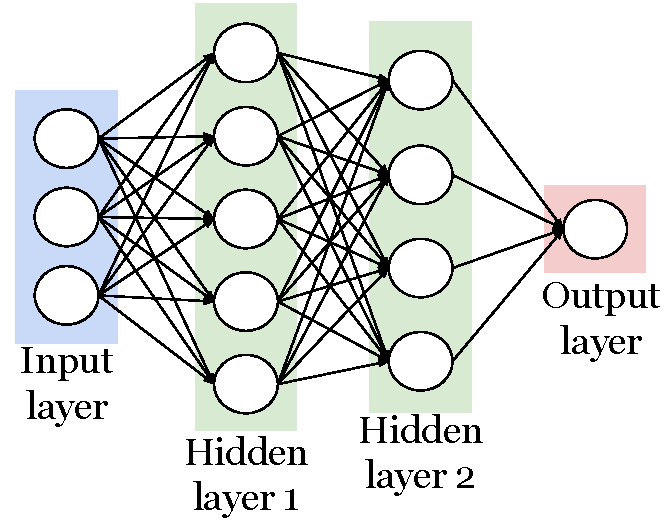
\includegraphics[width=0.6\textwidth]{images/neural_network.pdf}
    \end{center}
    \caption{Neural Network Schematic} \label{fig:neural_network}
\end{figure}

Deep convolutional neural networks (CNNs) which are very similar to ordinary Neural Networks that are discussed previously, have achieved breakthrough accuracies to image classification~\cite{lecun1990handwritten} that can easily be extended to the problem of facial expression recognition. Convolutional neural networks are made up of neurons that have learnable weights and biases. Each neuron receives an input performs a dot product and after that it performs a non-linear transformation. Deep CNNs are composed of several layers, and every layer transforms one volume of activations to another through a non linear differential function. Recent state-of-the-art architectures have used a number of additional components to enhance and complement the convolutional operation. The major components are:

\begin{itemize}
  \item Pooling layer
  \item ReLU layer~\cite{nair2010rectified}
  \item Dropout layer~\cite{srivastava2014dropout}
  \item Batch normalization~\cite{ioffe2015batch}
\end{itemize}

It is desirable to periodically introduce pooling layers between convolutional layers in order to reduce the spatial size of the image. The pooling layer operates on each local region of an image and computes the average of the pixel values in the region (Average pooling) or keeps the maximum pixel value of the region (Max pooling). The idea behind pooling is that makes CNNs invariant to variations in the representation of the image and reduces the effect of background. Also pooling reduces the number of trainable parameters and as a results the training of the network becomes faster. 

ReLU layer applies an elementwise activation function $\max(0,x)$, which turns negative values to zeros (thresholding at zero). 

Dropout layer provides a simple way to avoid overfitting. Overfitting is a phenomenon in which a model works well on the training dataset, but performs poorly on new unseen data. This happens since the model has learned both the signal and the noise from the training dataset. The idea behind dropout layers is to randomly set some activations to 0, essentially dropping components from a layer of the neural network. By doing this, the network is forced to find more ways to classify the images instead of over-depending on some features.

The idea behind batch normalisation is that instead of only normalising the input of the network, we normalise the inputs to layers within the network. Batch normalisation helps the network in many ways: networks train faster, allows higher learning rates, provides some regularisation, and makes weights easier to initialise. 

Figure~\ref{fig:CNN} depicts a simple convolutional neural network with convolutional layers, subsampling layers (pooling layers) followed by fully connected layers. We stack these three types of layers to form a Convolutional neural network architecture. The input is an image of dimensions $h\times w \times r$, where $h$ is the height, $w$ is the width, and $r$ is the number of channels, e.g $r=3$ for an RGB image and $r=1$ for a grayscale image. The convolutional layer has $k$ filters of size $m\times m \times d$, where $m$ is the filter size and obviously has to be smaller than the input image, and $d$ is equal to the depth of the input image, e.g for an RGB image $d=3$. The output is $k$ images of size $(h-m+1) \times (w-m+1)$. Usually an additive bias and and a non-linear activation function is applied to each image leaving the image  size unchanged. So the input to the next convolutional layer will be an image of size $(h-m+1) \times (w-m+1) \times k$. As mentioned before between the convolutional layers we insert a pooling layer that reduces the spatial size of the representation. After this operation the depth remains unchanged while the width and the height decrease proportional to the size of pooling layer $p$. After these layers we have any number of fully connected layers that have full connections to all activations from the previous layer as is the case to layers in a standard multilayer neural network. The fully connected layer uses a softmax activation function in the output layer. Putting it all together the convolutional and pooling layers act as feature extractors from the input image. For example first layers will learn edges and second layers will combine these edges in order to form more abstract representations like rectangular shapes. Next layers will combine these layers to create more abstract representations like a human eye or nose. So far we have described a feed-forward network that can be thought as a composition of a number of functions:
\begin{center}
$f(\mathbf{x;w}) = f_{L}(...f_{2}(f_{1}(\mathbf{x;w_{1}});\mathbf{w_{2}})...),\mathbf{w_{L}})$
\end{center}

Each function takes as input a data vector $\mathbf{x}_l$ where $l$ denotes the layer and and a parameter vector $\mathbf{w}_{l}$ and produces an output $\mathbf{x}_{l+1}$. The parameters $\mathbf{w} = (\mathbf{w_{1}, \mathbf{w}_{2},..., \mathbf{w}_{L}})$ for each layer $l$ are learned from the training dataset. In the case of image classification the data vectors $\mathbf{x}$ are 3D arrays of pixels (height, width, channels). The parameters $\mathbf{w} = (\mathbf{w_{1}, \mathbf{w}_{2},..., \mathbf{w}_{L}})$ should be learned in such a manner that the overall function $f(\mathbf{x;w})$ achieves a goal, that is minimising a loss function $L = l(\mathbf{z},\hat{\mathbf{z}})$ that expresses the penalty for predicting $\hat{\mathbf{z}}$ instead of $\mathbf{z}$. Learning will be achieved by adjusting the weights $\mathbf{w}$ such that the predicting $\hat{\mathbf{z}}$ is as close as possible to $\mathbf{z}$. The simplest algorithm to minimize $L$ is gradient descent\footnote{\url{https://en.wikipedia.org/wiki/Gradient_descent}}. The idea behind gradient descent is that you update the parameters $\mathbf{w}$ along the direction of the fastest descent of the loss function $L$. So the update of the parameters at every step $t$ is given by the following formula: 
\begin{center}
$\mathbf{w}^{t+1} = \mathbf{w}^{t} - \eta_{t}\frac{\partial f}{\partial \mathbf{w}}(\mathbf{w}^{t})$ \\
\text{where~$\eta_{t}$ is the learning rate at time step $t$}
\end{center}

The method used to train CNNs and which is based on gradient descent is called backpropagation\footnote{\url{https://en.wikipedia.org/wiki/Backpropagation}}. The idea is that the parameters of the models are adjusted in proportion to their contribution to the total error. So after this algorithm the architecture is able to classify correctly the images from the training dataset. Given that the training dataset is large enough, the architecture will generalise well to unseen images and classify them into correct categories. So in order to predict the category of a new image, the network will go through a forward propagation step with the optimal weights calculated by the backpropagation algorithm and will output a probability for each class. So the answer will be the category with the highest probability. 

\begin{figure}[t]
    \begin{center}
    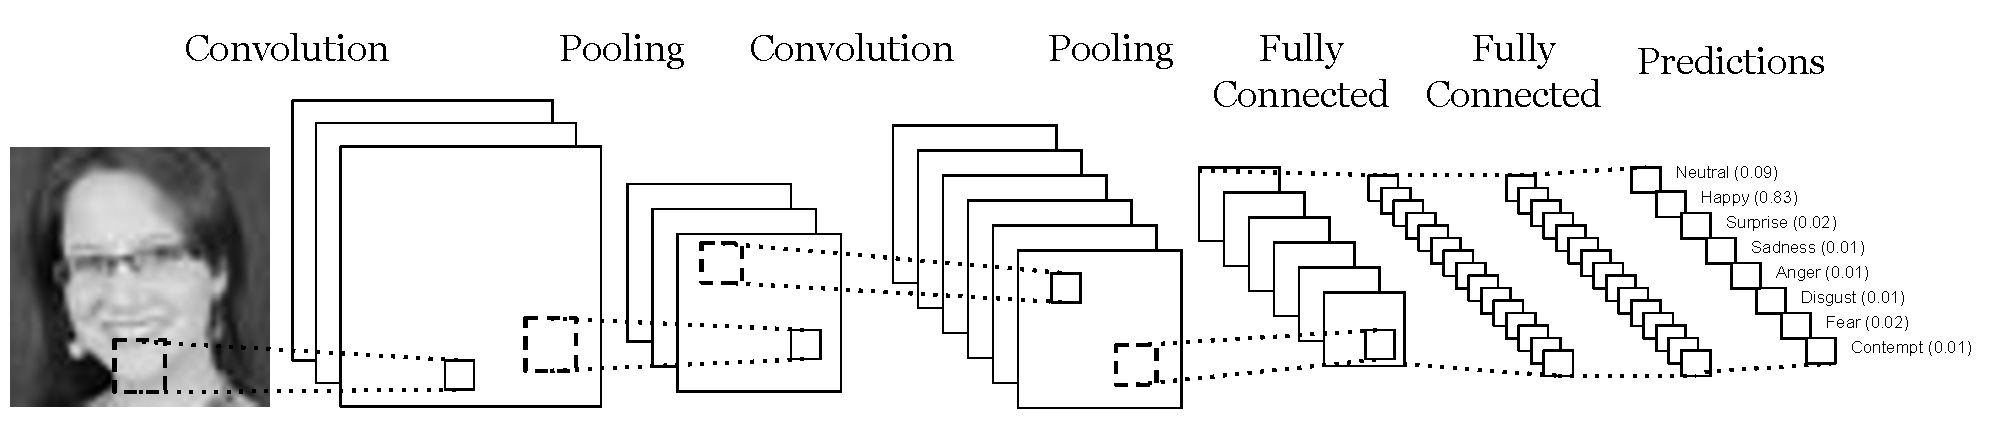
\includegraphics[width=1.0\textwidth]{images/CNN.pdf}
    \end{center}
    \caption{Convolutional Neural Network Schematic} \label{fig:CNN}
\end{figure}

In this paper, we experiment with the latest deep convolutional neural networks in order to classify human faces into discrete emotion labels. We train from scratch architectures including the VGG~\cite{simonyan2014very}, ResNet~\cite{he2016deep}, GoogLeNet~\cite{szegedy2015going}, DenseNet~\cite{huang2017densely}, and Wide ResNet~\cite{zagoruyko2016wide} networks. Also we experiment on transfer learning and multi-task learning. Transfer learning is a machine learning method where a model trained for a task is used as a starting point for a different task, while in multi-task learning multiple learning tasks are solved at the same time. Multiple CNNs are available such as VGG16 that are pre-trained on ImageNet~\cite{deng2009imagenet} or to perform facial recognition~\cite{parkhi2015deep}. These pre-trained models are used as feature extractors. With these features we train a linear support vector machine. Both high and low level features are taken from the pre-trained networks.
The rest of the paper is organized as follows. Related works are discussed in Section~\ref{ch:related work} and a description of the datasets used, in Section~\ref{ch:related work}. Section~\ref{ch:architectures} gives a brief description of the most popular CNN architectures, while sections~\ref{ch:transfer learning} and~\ref{ch:multi-task learning} present two popular methods that are used in deep learning. Section~\ref{ch:experiments and results} presents the experiments with their results, while section~\ref{ch:best algorithm} explains in detail the algorithm that achieves state-of-the-art accuracy on the FER+ dataset. Finally, section~\ref{ch:conclusion} gives an overview of our analysis.

%\afterpage{\blankpage}